%% Преамбула TeX-файла

% 1. Стиль и язык
\documentclass[utf8x, 14pt]{G7-32} % Стиль (по умолчанию будет 14pt)

% Остальные стандартные настройки убраны в preamble.inc.tex.
\sloppy

% Настройки стиля ГОСТ 7-32
% Для начала определяем, хотим мы или нет, чтобы рисунки и таблицы нумеровались в пределах раздела, или нам нужна сквозная нумерация.
\EqInChapter % формулы будут нумероваться в пределах раздела
\TableInChapter % таблицы будут нумероваться в пределах раздела
\PicInChapter % рисунки будут нумероваться в пределах раздела

% Добавляем гипертекстовое оглавление в PDF
\usepackage[
bookmarks=true, colorlinks=true, unicode=true,
urlcolor=black,linkcolor=black, anchorcolor=black,
citecolor=black, menucolor=black, filecolor=black,
]{hyperref}
\usepackage{pgfplots}
\usepackage{nomencl}

\usepackage{float}

\usepackage{indentfirst}
\setlength{\parindent}{1.25cm}

\AfterHyperrefFix

\usepackage{microtype}% полезный пакет для микротипографии, увы под xelatex мало чего умеет, но под pdflatex хорошо улучшает читаемость

% Тире могут быть невидимы в Adobe Reader
\ifInvisibleDashes
\MakeDashesBold
\fi

% Для псевдокода
\usepackage{algorithm}
\usepackage{algpseudocode}

\usepackage{graphicx}   % Пакет для включения рисунков
\usepackage[final]{pdfpages}
% С такими оно полями оно работает по-умолчанию:
% \RequirePackage[left=20mm,right=10mm,top=20mm,bottom=20mm,headsep=0pt,includefoot]{geometry}
% Если вас тошнит от поля в 10мм --- увеличивайте до 20-ти, ну и про переплёт не забывайте:
\geometry{right=10mm}
\geometry{left=30mm}
\geometry{bottom=20mm}
\geometry{top=19mm}
\geometry{ignorefoot}% считать от нижней границы текста


% Пакет Tikz
\usepackage{tikz}
\usetikzlibrary{arrows,positioning,shadows}

% Произвольная нумерация списков.
\usepackage{enumerate}

% ячейки в несколько строчек
\usepackage{multirow}

% itemize внутри tabular
\usepackage{paralist,array}

%\setlength{\parskip}{1ex plus0.5ex minus0.5ex} % разрыв между абзацами
\setlength{\parskip}{1.5ex} % разрыв между абзацами
\usepackage{blindtext}

\usepackage{setspace}
\setstretch{1.5}

% Для таблиц
\usepackage[para,online,flushleft]{threeparttable}

% Центрирование подписей к плавающим окружениям
%\usepackage[justification=centering]{caption}

\usepackage{newfloat}
\DeclareFloatingEnvironment[
placement={!ht},
name=Equation
]{eqndescNoIndent}
\edef\fixEqndesc{\noexpand\setlength{\noexpand\parindent}{\the\parindent}\noexpand\setlength{\noexpand\parskip}{\the\parskip}}
\newenvironment{eqndesc}[1][!ht]{%
    \begin{eqndescNoIndent}[#1]%
\fixEqndesc%
}
{\end{eqndescNoIndent}}

\usepackage{afterpage}

\newcommand\blankpage{
	\null
	\thispagestyle{empty}
	\newpage
}



% Настройки листингов.
\ifPDFTeX
% 8 Листинги

\usepackage{listings}

% Значения по умолчанию
\lstset{
  basicstyle= \footnotesize,
  breakatwhitespace=true,% разрыв строк только на whitespacce
  breaklines=true,       % переносить длинные строки
%   captionpos=b,          % подписи снизу -- вроде не надо
  inputencoding=koi8-r,
  numbers=left,          % нумерация слева
  numberstyle=\footnotesize,
  showspaces=false,      % показывать пробелы подчеркиваниями -- идиотизм 70-х годов
  showstringspaces=false,
  showtabs=false,        % и табы тоже
  stepnumber=1,
  tabsize=4,              % кому нужны табы по 8 символов?
  frame=single,
  xleftmargin=2.4em,
  framexleftmargin=2em
}

% Стиль для псевдокода: строчки обычно короткие, поэтому размер шрифта побольше
\lstdefinestyle{pseudocode}{
  basicstyle=\small,
  keywordstyle=\color{black}\bfseries\underbar,
  language=Pseudocode,
  numberstyle=\footnotesize,
  commentstyle=\footnotesize\it
}

% Стиль для обычного кода: маленький шрифт
\lstdefinestyle{realcode}{
  basicstyle=\scriptsize,
  numberstyle=\footnotesize
}

% Стиль для коротких кусков обычного кода: средний шрифт
\lstdefinestyle{simplecode}{
  basicstyle=\footnotesize,
  numberstyle=\footnotesize
}

% Стиль для BNF
\lstdefinestyle{grammar}{
  basicstyle=\footnotesize,
  numberstyle=\footnotesize,
  stringstyle=\bfseries\ttfamily,
  language=BNF
}

% Определим свой язык для написания псевдокодов на основе Python
\lstdefinelanguage[]{Pseudocode}[]{Python}{
  morekeywords={each,empty,wait,do},% ключевые слова добавлять сюда
  morecomment=[s]{\{}{\}},% комменты {а-ля Pascal} смотрятся нагляднее
  literate=% а сюда добавлять операторы, которые хотите отображать как мат. символы
    {->}{\ensuremath{$\rightarrow$}~}2%
    {<-}{\ensuremath{$\leftarrow$}~}2%
    {:=}{\ensuremath{$\leftarrow$}~}2%
    {<--}{\ensuremath{$\Longleftarrow$}~}2%
}[keywords,comments]

% Свой язык для задания грамматик в BNF
\lstdefinelanguage[]{BNF}[]{}{
  morekeywords={},
  morecomment=[s]{@}{@},
  morestring=[b]",%
  literate=%
    {->}{\ensuremath{$\rightarrow$}~}2%
    {*}{\ensuremath{$^*$}~}2%
    {+}{\ensuremath{$^+$}~}2%
    {|}{\ensuremath{$|$}~}2%
}[keywords,comments,strings]

% Подписи к листингам на русском языке.
\renewcommand\lstlistingname{Листинг}
\renewcommand\lstlistlistingname{Листинги}

\else
\usepackage{local-minted}
\fi

% Стиль титульного листа и заголовки
% \include{00-title}


\begin{document}

\pagenumbering{arabic}
\setcounter{page}{2}
\frontmatter % выключает нумерацию ВСЕГО; здесь начинаются ненумерованные главы: реферат, введение, глоссарий, сокращения и прочее.

%\maketitle %создает титульную страницу
% \afterpage{\blankpage}\afterpage{\blankpage}\afterpage{\blankpage}
% пропущены страницы под тз и план (у меня их 2 тз и 1 план, итого 3, вам надо пропустить столько, сколько страниц у вас в тз и плане)


%\listoffigures                         % Список рисунков

%\listoftables                          % Список таблиц

%\NormRefs % Нормативные ссылки 
% Команды \breakingbeforechapters и \nonbreakingbeforechapters
% управляют разрывом страницы перед главами.
% По-умолчанию страница разрывается.
% \include{11-referat}
% \nobreakingbeforechapters
% \breakingbeforechapters

\tableofcontents

% \printnomenclature % Автоматический список сокращений

\Introduction

Обеспечение безопасного доступа к файлам в операционной системе Linux является актуальной задачей.  
При работе с файлами и каталогами в Linux необходимо обеспечивать конфиденциальность данных и предоставлять защиту от вредоносных действий.

Данная курсовая работа посвящена разработке модуля, позволяющего ограничивать операции к определенным файлам, каталогам.

\mainmatter % это включает нумерацию глав и секций в документе ниже

\chapter{Аналитический раздел}
\label{cha:analysis}

\section{Постановка задачи}

В соответствии с заданием на курсовую работу необходимо разработать загружаемый модуль ядра для ОС Linux, позволяющий скрывать файлы или запрещать их изменение, чтение и удаление. Также обеспечить 
запрещать удаление, переименование каталогов. Предусмотреть возможность ввода пароля для разрешения операций над ними. Предоставить пользователю возможность задавать список таких файлов.

Для решения поставленной задачи необходимо:

\begin{itemize}
	\item проанализировать возможности перехвата функций ядра Linux;
	\item выбрать системные вызовы, которые необходимо перехватить;
	\item разработать алгоритм перехвата, алгоритмы hook--функций и структуру программного обеспечения;
	\item реализовать программное обеспечение;
	\item исследовать работу ПО.
\end{itemize}

\section{Способы перехвата функций ядра}

\subsection{ftrace}

ftrace предоставляет возможности для трассировки функций.  С его помощью можно отслеживать контекстные переключения, измерять время обработки прерываний, высчитывать время на активизацию заданий с высоким приоритетом и многое другое \cite{ftrace}.

Ftrace был разработан Стивеном Ростедтом и добавлен в ядро в 2008 году, начиная с версии 2.6.27. Ftrace --- фреймворк, предоставляющий отладочный кольцевой буфер для записи данных. Собирают эти данные встроенные в ядро программы--трассировщики \cite{ftrace}.

Работает ftrace на базе файловой системы debugfs, которая в большинстве современных дистрибутивов Linux смонтирована по умолчанию. 

Каждую перехватываемую функцию можно описать следующей структурой:

\begin{lstlisting}[label=code:ftracehook,caption=Структура ftrace\_hook]
struct ftrace_hook {
	const char *name;
	void *function;
	void *original;
	
	unsigned long address;
	struct ftrace_ops ops;
};
\end{lstlisting}

Поля структуры:

\textit{name} --- имя перехватываемой функции;

\textit{function} ---  адрес функции--обертки, которая будет вызываться вместо перехваченной функции;

\textit{original} ---  указатель на место, куда следует записать адрес перехватываемой функции, заполняется при установке;

\textit{address} --- адрес перехватываемой функции, заполняется при установке;

\textit{ops} --- служебная информация ftrace.

\begin{lstlisting}[label=code:ftracehookexm,caption=Пример заполнения структуры ftrace\_hook]
#define HOOK(_name, _function, _original)       \
{                                       \
	.name = (_name),                    \
	.function = (_function),            \
	.original = (_original),            \
}
	
static struct ftrace_hook hooked_functions[] = {
	HOOK("sys_clone",   fh_sys_clone,   &real_sys_clone),
	HOOK("sys_execve",  fh_sys_execve,  &real_sys_execve),
};
\end{lstlisting}

\subsection{kprobes}

Kprobes --- специализированное API, в первую очередь предназначенное для отладки и трассирования ядра \cite{stiven}. Этот интерфейс позволяет устанавливать пред- и постобработчики для любой инструкции в ядре, а также обработчики на вход и возврат из функции. Обработчики получают доступ к регистрам и могут их изменять.

Kprobes реализуются с помощью точек останова (инструкции int3), внедряемых в исполнимый код ядра, что позволяет устанавливать kprobes в любом месте любой функции, если оно известно. Аналогично, kretprobes реализуются через подмену адреса возврата на стеке и позволяют перехватить возврат из любой функции.

При использовании kprobes для получения аргументов функции или значений локальных переменных надо знать, в каких регистрах или где на стеке они лежат, и самостоятельно их оттуда извлекать. Для решения данной проблемы существует jprobes ---  надстройка над kprobes, самостоятельно извлекающая аргументы функции из регистров или стека и вызывающая обработчик, который должен иметь ту же сигнатуру, что и перехватываемая функция. Однако jprobes объявлен устаревшим и удален из современных ядер.

\subsection{ Linux Security API}

Linux Security API --- интерфейс, созданный для перехвата функций ядра. В критических местах кода ядра расположены вызовы security--функций, которые в свою очередь вызывают коллбеки, установленные security--модулем. Security--модуль может анализировать контекст операции и принимать решение о ее разрешении или запрете.

Для Linux Security API характерны следующие ограничения:
\begin{itemize}
	\item security--модули не могут быть загружены динамически, они являются частью ядра и требуют его перекомпиляции;
	\item в системе может быть только один security--модуль.
\end{itemize}

%Если по поводу множественности модулей позиция разработчиков ядра неоднозначная, то запрет на динамическую загрузку принципиальный: security-модуль должен быть частью ядра, чтобы обеспечивать безопасность постоянно, с момента загрузки.

Таким образом, для использования Security API необходимо поставлять собственную сборку ядра, а также интегрировать дополнительный модуль с SELinux или AppArmor, которые используются популярными дистрибутивами. 

\subsection{Модификация таблицы системных вызовов}

В ядре Linux все обработчики системных вызовов хранятся в таблице sys\_call\_table \cite{linux}. Подмена значений в этой таблице приводит к смене поведения всей системы. Таким образом, сохранив старое значения обработчика и подставив в таблицу собственный обработчик, можно перехватить системный вызов.

Однако данный подход обладает следующими недостатками:
\begin{itemize}
	\item Техническая сложность реализации, заключающаяся в необходимости обхода защиты от модификации таблицы, атомарное и безопасное выполнение замены.
	\item Невозможность перехвата некоторых обработчиков. В ядрах до версии 4.16 обработка системных вызовов для архитектуры x86\_64 содержала целый ряд оптимизаций. Некоторые из них требовали того, что обработчик системного вызова являлся специальным переходником, реализованным на ассемблере. Соответственно, подобные обработчики порой сложно, а иногда и вовсе невозможно заменить на собственные, написанные на Си \cite{all}.
\end{itemize}

\subsection{Cплайсинг}

Сплайсинг заключается в замене инструкций в начале функции на безусловный переход, ведущий в обработчик. Оригинальные инструкции переносятся в другое место и исполняются перед переходом обратно в перехваченную функцию. Именно таким образом реализуется jump--оптимизация для kprobes. Используя сплайсинг, можно добиться тех же результатов, но без дополнительных расходов на kprobes и с полным контролем ситуации.

Сложность использования сплайсинга заключается в необходимости синхронизации установки и снятия перехвата, обхода защиты от модификации регионов памяти с кодом, инвалидации кешей процессора после замены инструкций, дизассемблировании заменяемых инструкций и проверки на отсутствие переходов внутрь заменяемого кода.


%\section{Перехват функций ядра с помощью ptrace}

%ptrace() --- это системный вызов, который дает возможность одному процессу управлять исполнением другого. Он так же позволяет изменять содержимое памяти трассируемого процесса. Трассируемый процесс ведет себя как обычно до тех пор пока не получит сигнал. Когда это происходит, процесс переходит в состояние останова, а процесс--трассировщик информируется об этом вызовом wait(). После этого процесс--трассировщик, через вызовы ptrace, определяет реакцию трассируемого процесса. Исключение составляет сигнал SIGKILL, который уничтожает процесс.

%Кроме того, можно задать переход трассируемого процесса в состояние останова по определенному событию, которое возникло в ходе его исполнения. Это происходит только в том случае, если процесс--трассировщик установил какие--либо флаги событий в контексте трассируемого процесса. Трассировщик также может завершить трассируемый процесс, установив при этом код его завершения. После выполнения каких--либо действий трассировщик может завершить отлаживаемый процесс или продолжить его исполнение.

%Объявление ptrace() представлено в листинге \ref{code:ptrace}.

%\begin{lstlisting}[label=code:ptrace,caption=Функция ptrace]
%#include <sys/ptrace.h>

%long  int ptrace(enum __ptrace_request request, pid_t pid, void * addr, void * data)
%\end{lstlisting}

%Вызову передаются четыре аргумента, где \textit{request} определяет что необходимо сделать, \textit{pid} --- идентификатор трассируемого процесса, \textit{addr} --- смещение в пользовательском пространстве трассируемого процесса, откуда будет прочитано слово данных и возвращено в качестве результата работы вызова.

% Родительский процесс может породить дочерний процесс и выполнять его трассировку посредством вызова ptrace с аргументом request, имеющим значение PTRACE\_TRACEME. Процесс--трассировщик может выполнять трассировку уже существующего процесса, используя значение PTRACE\_ATTACH.


\subsection{Сравнительный анализ способов перехвата}

Результаты сравнения различных способов перехвата функций ядра представлены в таблице \ref{tbl:compare}

\clearpage

\begin{table}[h]
	\begin{center}
		\begin{threeparttable}
			\captionsetup{justification=raggedright,singlelinecheck=off}
			\caption{\label{tbl:compare} Результаты сравнения}
			\begin{tabular}{|p{2.9cm}|p{3cm}|p{3cm}|p{3cm}|p{3.2cm}|}
				\hline
				Способ перехвата & Необходимость перекомпиляции ядра & Возможность перехвата любых обработчиков & Доступ к аргументам функции через переменные & Необходимость обхода защиты от модификации регионов памяти\\  \hline
				Linux Security API & да & нет & да &  нет \\ \hline 
				Модификация таблиц системных вызовов & нет & нет & да  & да \\ \hline 
				kprobes & нет & да & нет & нет  \\ \hline 
				Сплайсинг & нет & да& да &  да \\ \hline 
				ftrace & нет & да & да & нет \\ \hline 
			\end{tabular}
		\end{threeparttable}
	\end{center}
\end{table}


\section{Перехватываемые функции ядра}

% К операциям файлового ввода--вывода относятся открытие файла, чтение из файла, запись в файл и так далее. 

% Все открытые файлы представлены в ядре файловыми дескрипторами. Когда процесс открывает существующий файл или создает новый, ядро возвращает ему файловый дескриптор \cite{stiven}.

%В соответствии с принятыми соглашениями командные оболочки UNIX ассоциируют файловый дескриптор 0 со стандартным устройством ввода процесса, 1 --- со стандартным устройством вывода и 2 --- со стандартным устройством вывода сообщений об ошибках.

\subsection{Функция getdents64}

Для сокрытия файла необходимо перехватить функцию ядра getdents64, так как она возвращает записи каталога. 
\begin{lstlisting}[label=code:getdents64,caption=Функции getdents64]
#include <fcntl.h>
	
int getdents64(unsigned int fd, struct linux_dirent64 *dirp, unsigned int count);
\end{lstlisting}

Системный вызов getdents64 читает несколько структур linux\_dirent64 из каталога, на который указывает открытый файловый дескриптор fd, в буфер, указанный в dirp. В аргументе count задается размер этого буфера.

Структура linux\_dirent64 определена следующим образом:
\clearpage
\begin{lstlisting}[label=code:linuxdirent64,caption=Структура linux\_dirent64]
struct linux_dirent64 {
		ino64_t		d_ino;
		off64_t		d_off;    
		unsigned short	d_reclen; 
		unsigned char	d_type;  
		char	d_name[]; 
};
\end{lstlisting}

В d\_ino указан номер inode. В d\_off задается расстояние от начала каталога до начала следующей linux\_dirent64. В d\_reclen указывается размер данного linux\_dirent64. В d\_name задается имя файла, в d\_type --- тип файла.
 
Таким образом, перехват системного вызова getdents64 позволяет удалить запись из списка записей каталога.
Перехват вызова осуществляется при помощи создания указателя на системный вызов getdents64.

\begin{lstlisting}[label=code:getdents_p,caption=Указатель на getdents64]
static asmlinkage long (*real_sys_getdents64)(const struct pt_regs *);
\end{lstlisting}

\subsection{Функция unlink}

Удаление записей из каталога производится с помощью функции unlink.

\begin{lstlisting}[label=code:unlink,caption=Функция unlink]
#include <unistd.h>

int unlink(const char *pathname);
\end{lstlisting}

Эта функция удаляет запись из файла каталога и уменьшает значение счетчика ссылок на файл pathname. Если на файл указывает несколько ссылок, то его содержимое будет через них по--прежнему доступно.

Таким образом, для того, чтобы запретить удаление файла, необходимо перехватить системный вызов unlink.
Перехват вызова осуществляется при помощи создания указателя на системный вызов.

\begin{lstlisting}[label=code:unlink_p,caption=Указатель на unlink]
static asmlinkage long (*real_sys_unlink) (struct pt_regs *regs);
\end{lstlisting}



\subsection{Функции open}
Чтение из файла и запись в него производится с помощью функции open.

\begin{lstlisting}[label=code:open,caption=Функция open]
#include <fcntl.h>

int open(const char *pathname, int flags, ...
                  /* mode_t mode */ );
\end{lstlisting}
Для того, чтобы запретить чтение из файла и запись в него, необходимо перехватить системные вызовы open.
Перехват осуществляется при помощи создания указателей на системные вызовы.

\begin{lstlisting}[label=code:unlink_p,caption=Указатели на open{,} write и read.]
static asmlinkage long (*real_sys_open)(struct pt_regs *regs);
\end{lstlisting}


\subsection{Функция rename}
Переименование файла и каталога производится с помощью функции rename.

\begin{lstlisting}[label=code:rename,caption=Функция rename]
#include <fcntl.h>

int rename(const char *oldpath, const char *newpath);
\end{lstlisting}
Для того, чтобы запретить переименовать файла и каталога, необходимо перехватить системные вызовы rename.
Перехват осуществляется при помощи создания указателей на системные вызовы.

\begin{lstlisting}[label=code:rename_p,caption=Указатели на rename]
static asmlinkage long (*real_sys_rename)(struct pt_regs *regs);
\end{lstlisting}



\section*{Вывод}

В результате сравнительного анализа выбран способ перехвата функций ядра --- ftrace, так как он позволяет перехватывать любые функции ядра и не требует его перекомпиляции.
Для сокрытия файла необходимо перехватить функцию getdents64, для переименования --- функция rename, для запрета чтения из файла и записи в файл --- функция open, удаления --- unlink.
\chapter{Конструкторский раздел}
\label{cha:design}

\section{IDEF0}

На рисунке \ref{fig:idef0} приведена диаграмма состояний IDEF0 нулевого уровня, а на рисунке \ref{fig:idef1} --- диаграмма состояний IDEF0 первого уровня.

\begin{figure}[ph!]
	\center{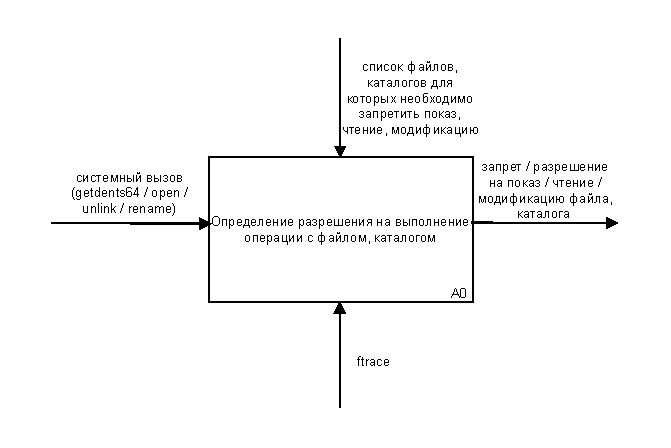
\includegraphics[scale=1.3]{img/idef0_0.pdf}}
	\caption{Диаграмма состояний IDEF0 нулевого уровня}
	\label{fig:idef0}
\end{figure}

\begin{figure}[ph!]
	\center{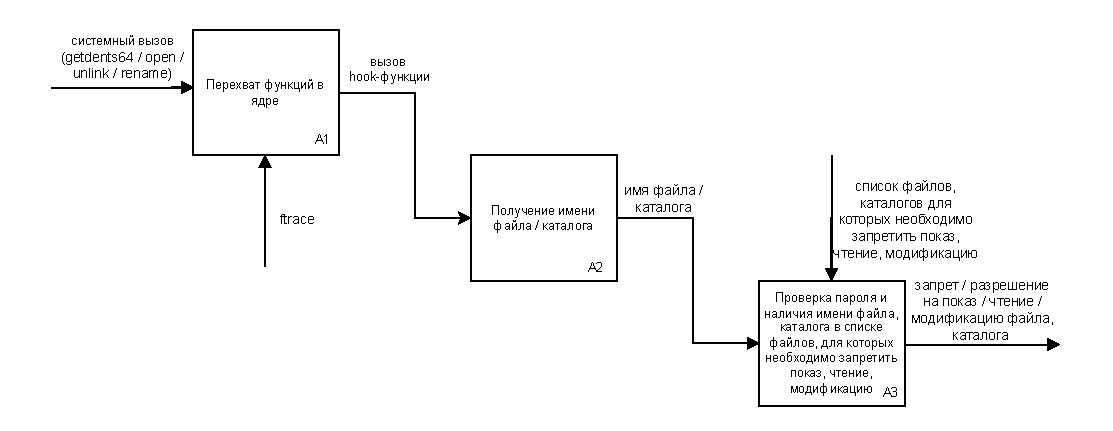
\includegraphics[scale=0.9]{img/idef0_1.pdf}}
	\caption{Диаграмма состояний IDEF0 первого уровня}
	\label{fig:idef1}
\end{figure}

\clearpage

%\section{Алгоритм создания символьного устройства}

%На рисунке \ref{fig:dev} приведена схема создания символьного устройства для ввода пароля.

%\begin{figure}[ph!]
%	\center{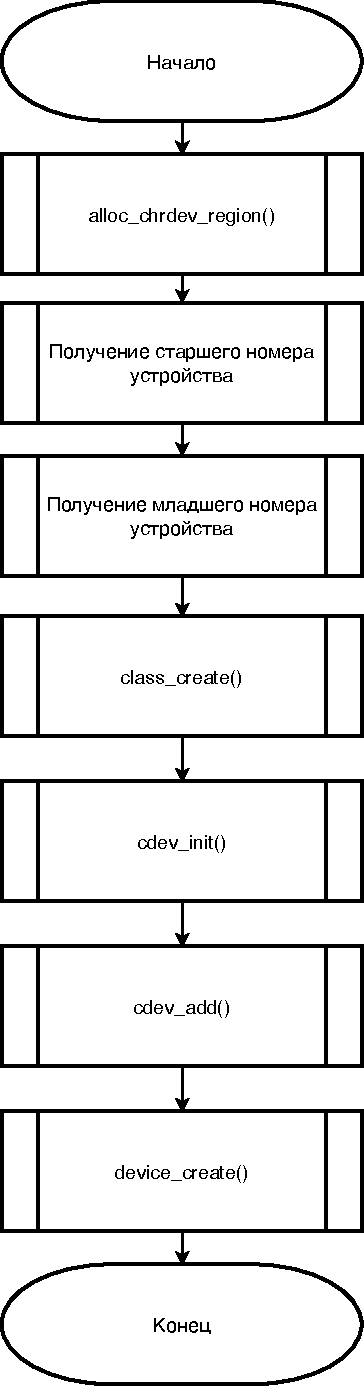
\includegraphics[scale=0.65]{img/cdev.pdf}}
%	\caption{Алгоритм создания символьного устройства}
%	\label{fig:dev}
%\end{figure}

%\clearpage

%\section{Алгоритм проверки наличия разрешения на выполнение действия с файлом}

%На рисунке \ref{fig:init} приведена схема алгоритма проверки наличия разрешения на выполнение действия с файлом.

%\begin{figure}[ph!]
%	\center{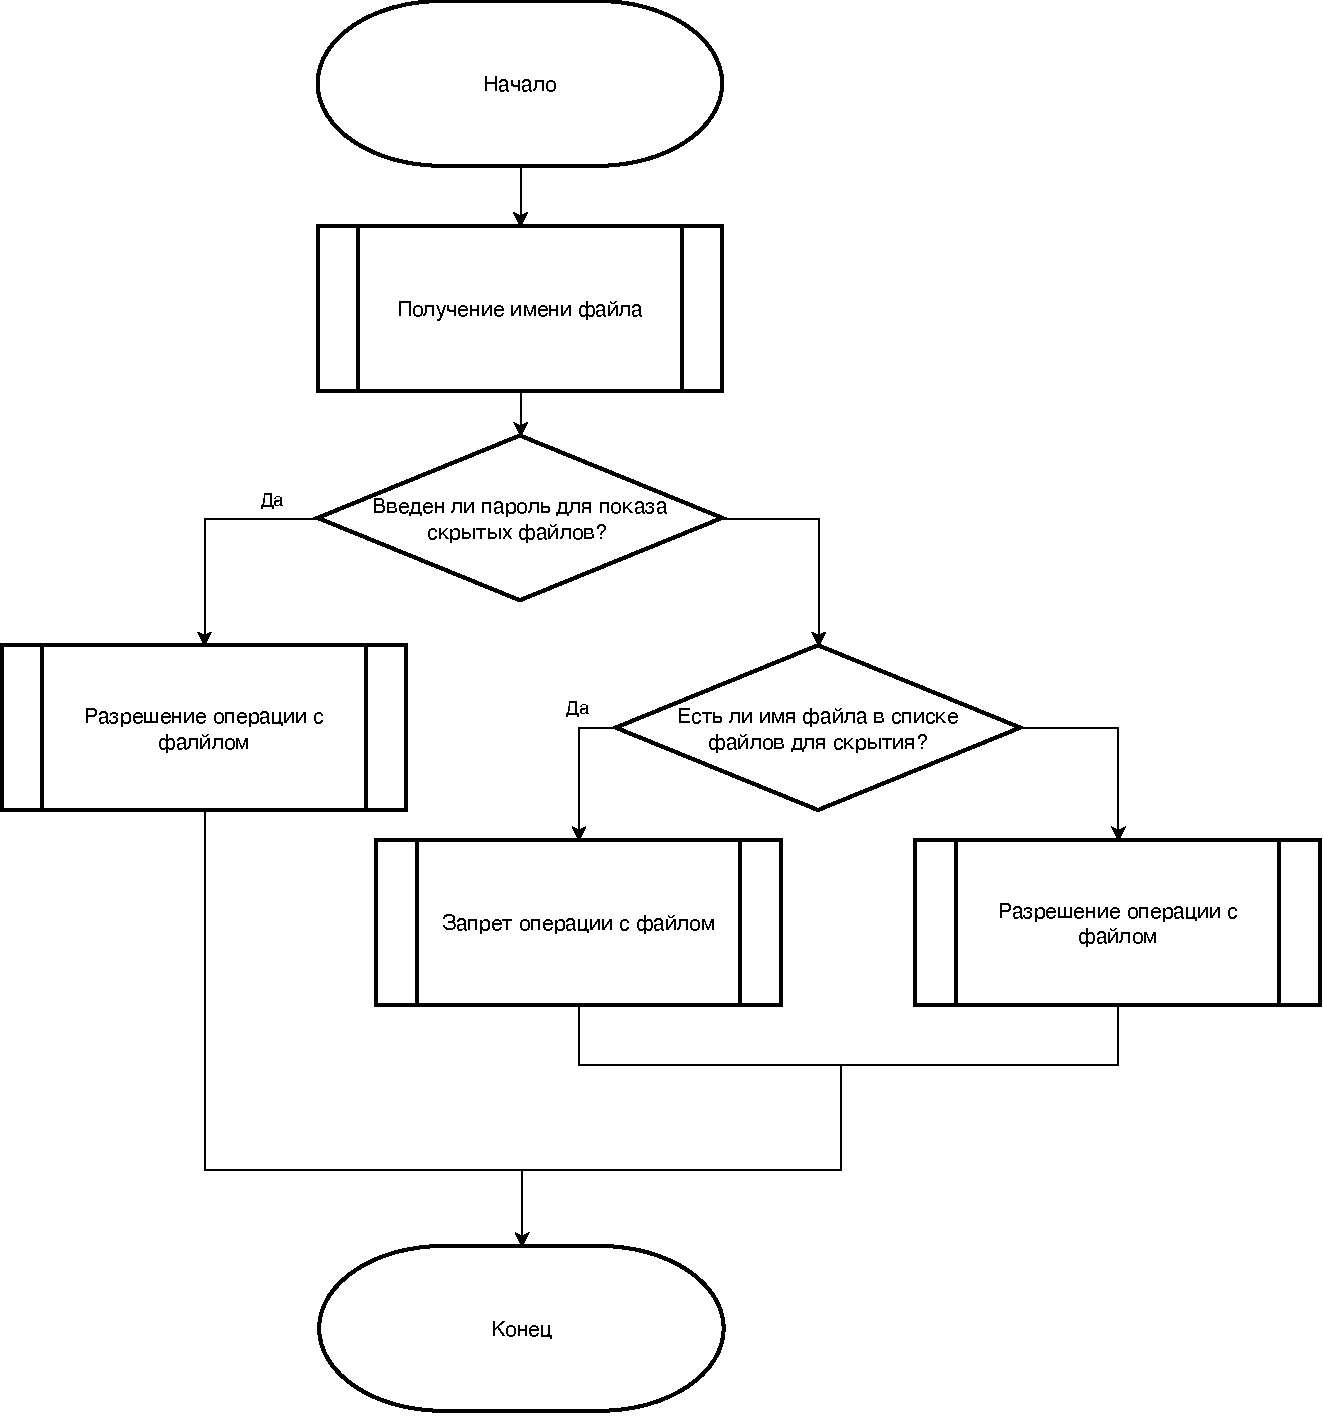
\includegraphics[scale=0.6]{img/check.pdf}}
%	\caption{Алгоритм проверки наличия разрешения на выполнение действия с файлом}
%	\label{fig:init}
%\end{figure}

%\clearpage

\section{Алгоритм проверки необходимости сокрытия файла}

На рисунке \ref{fig:getdents64} приведена схема алгоритма проверки необходимости сокрытия файла.

\begin{figure}[ph!]
	\center{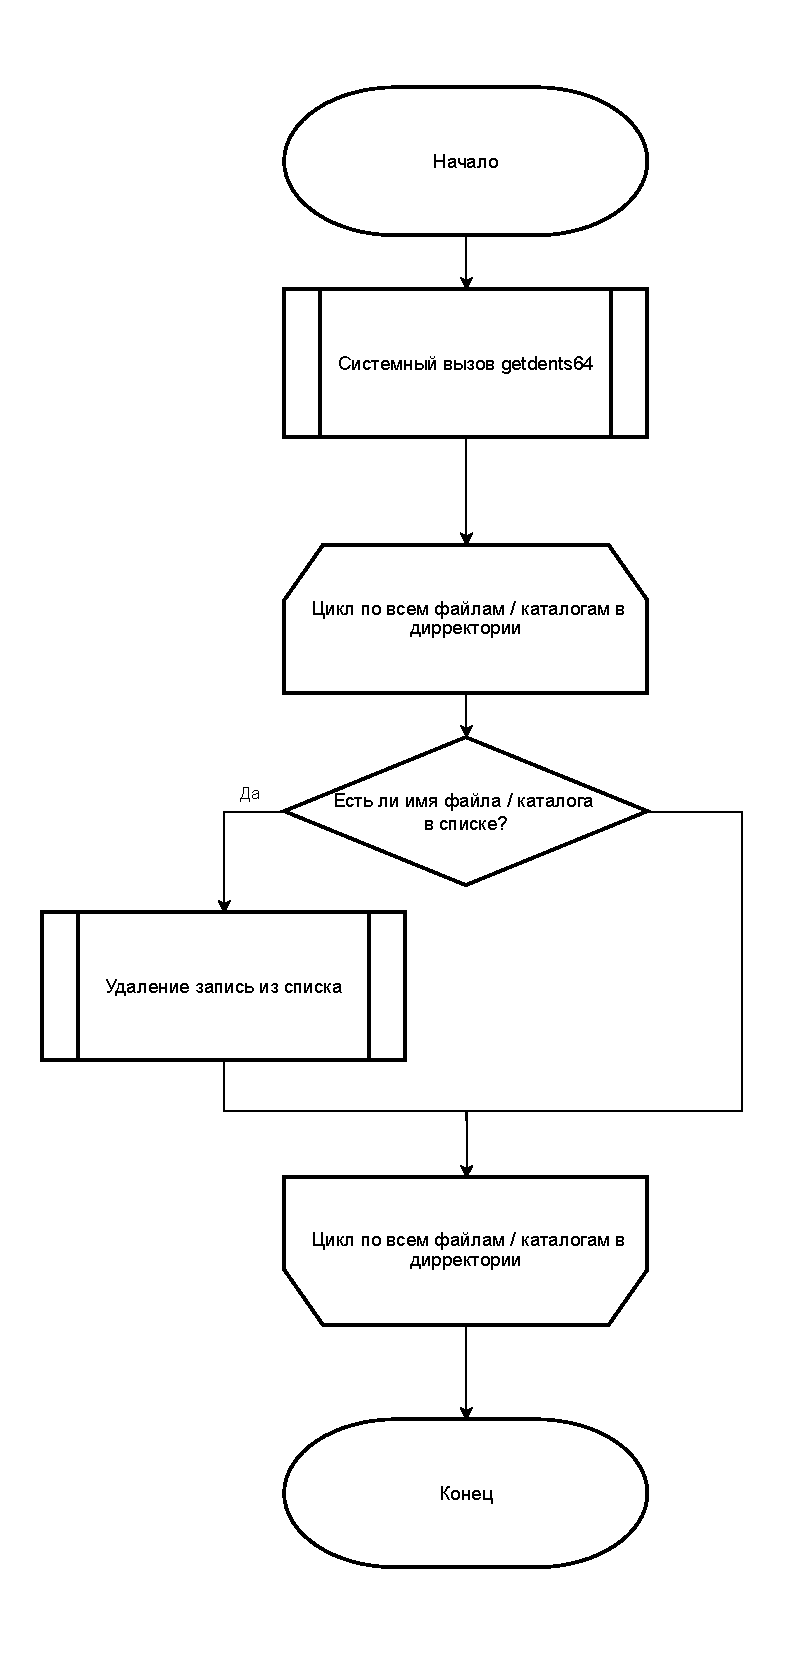
\includegraphics[scale=0.65]{img/getdents.pdf}}
	\caption{Алгоритм проверки необходимости сокрытия файла}
	\label{fig:getdents64}
\end{figure}

\clearpage

\section{Алгоритм проверки разрешения на удаление файла}

На рисунке \ref{fig:unlink} приведена схема алгоритма проверки разрешения на удаление файла.

\begin{figure}[ph!]
	\center{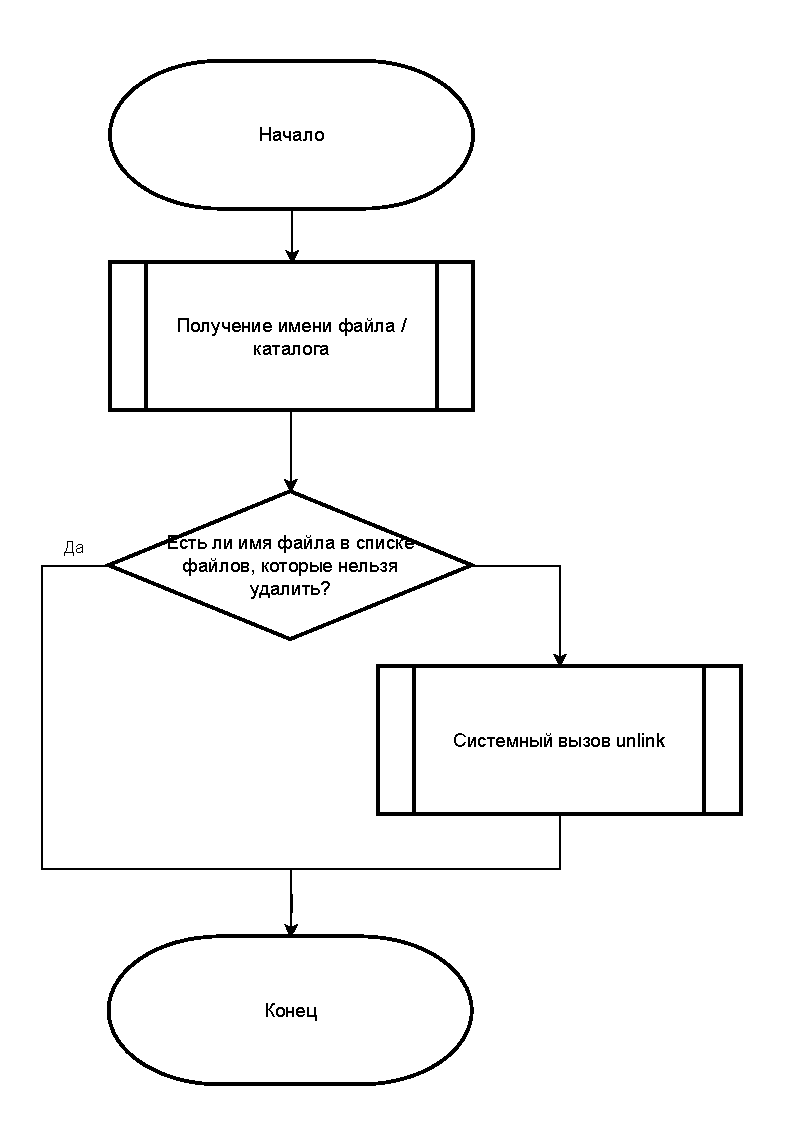
\includegraphics[scale=0.65]{img/unlink.pdf}}
	\caption{Алгоритм проверки разрешения на удаления файла}
	\label{fig:unlink}
\end{figure}

\clearpage

\section{Алгоритм проверки разрешения на переименование файла и каталога}

На рисунке \ref{fig:rename} приведена схема алгоритма проверки разрешения на чтение из файла.

\begin{figure}[ph!]
	\center{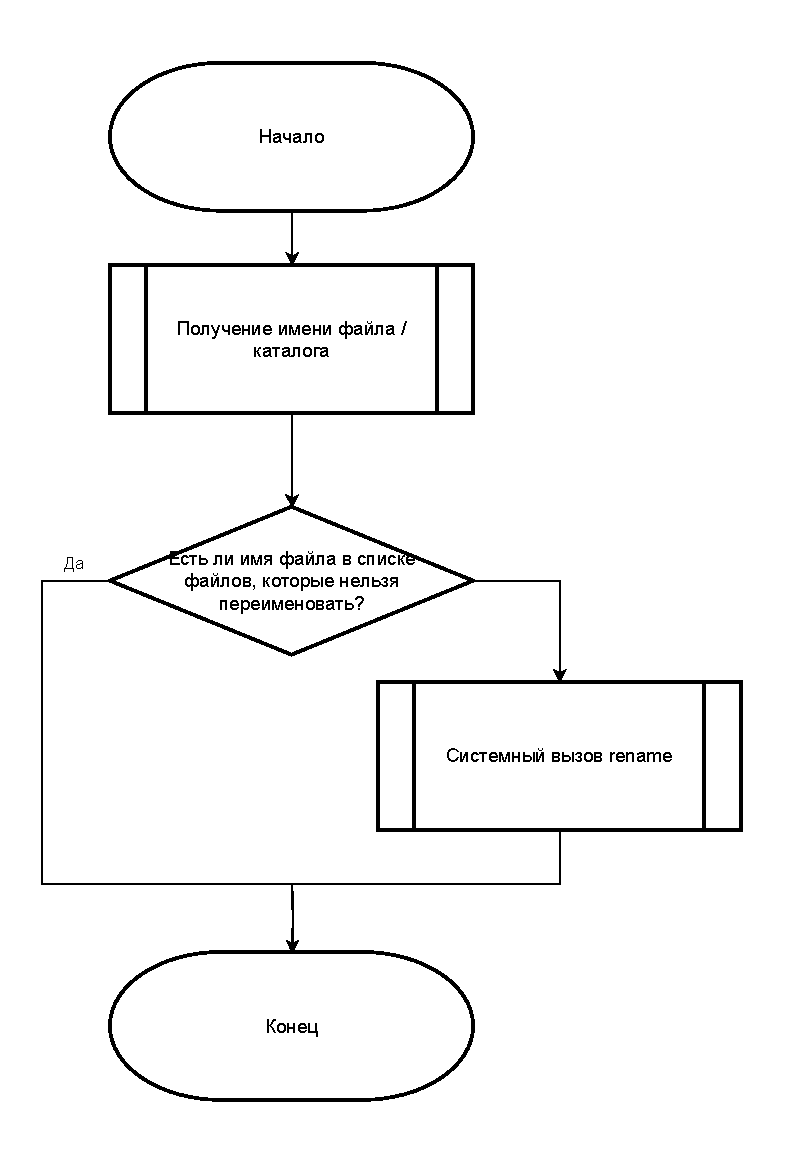
\includegraphics[scale=0.52]{img/rename.pdf}}
	\caption{Алгоритм проверки разрешения на чтение из файла}
	\label{fig:rename}
\end{figure}

\section{Алгоритм проверки разрешения на чтение и запись}

На рисунке \ref{fig:readwrite} приведена схема алгоритма проверки разрешения на чтение из файла и запись в него.

\begin{figure}[ph!]
	\center{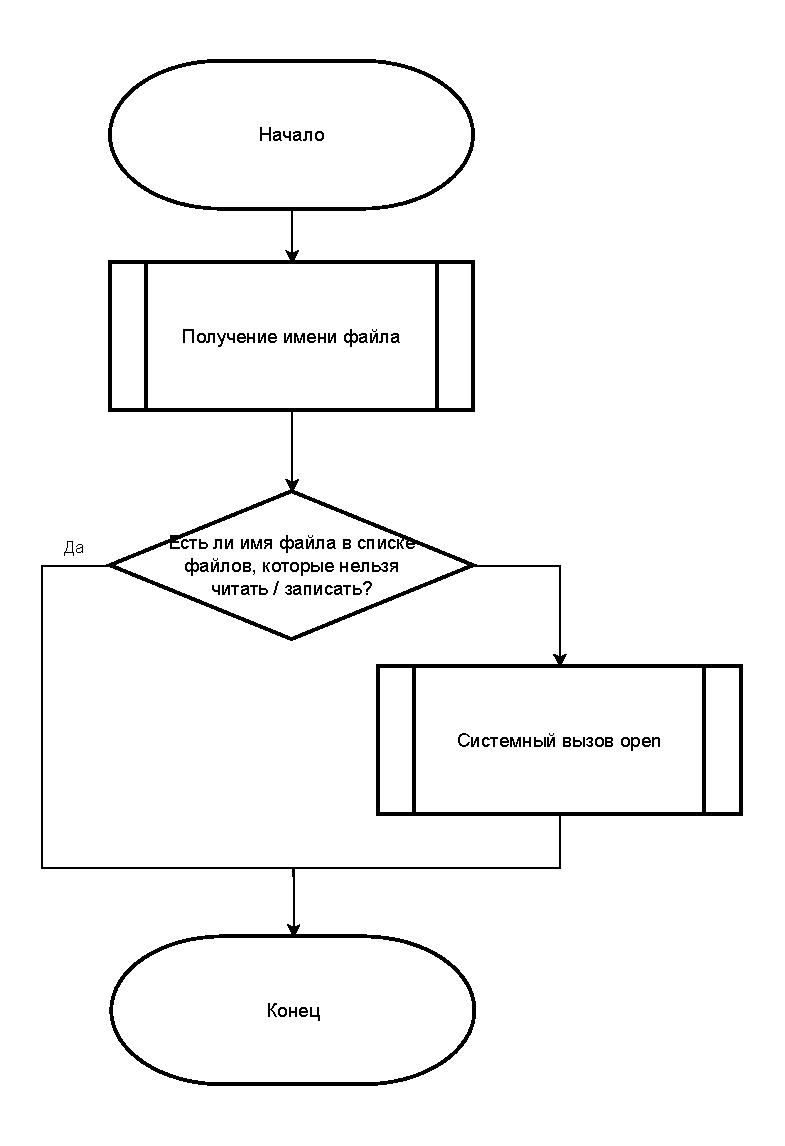
\includegraphics[scale=0.52]{img/readwrite.pdf}}
	\caption{Алгоритм проверки разрешения на чтение из файла и запись в него}
	\label{fig:readwrite}
\end{figure}

\clearpage

\section{Структура программного обеспечения}

На рисунке \ref{fig:struct} представлена структура программного обеспечения.

\begin{figure}[ph!]
	\center{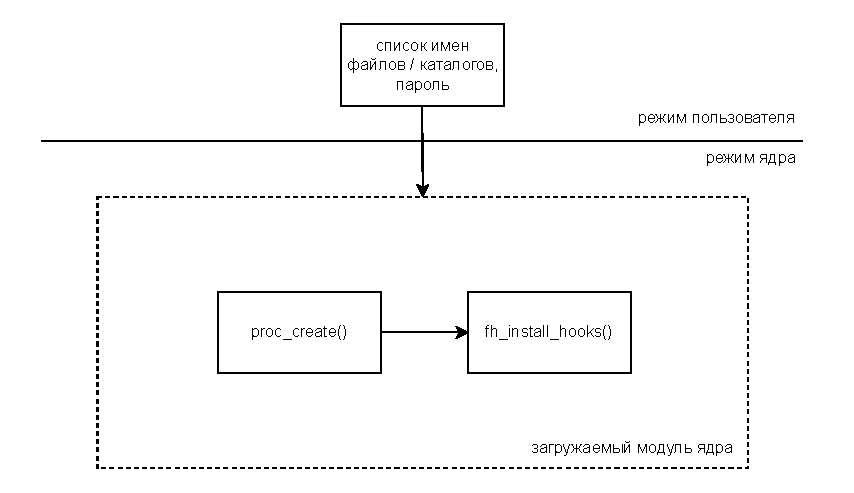
\includegraphics[scale=1]{img/structure.pdf}}
	\caption{Структура программного обеспечения}
	\label{fig:struct}
\end{figure}




\chapter{Технологический раздел}
\label{cha:impl}

\section{Выбор языка и среды программирования}

В качестве языка программирования был выбран язык Си. Для сборки модуля использовалась утилита make. В качестве среды программирования был выбран VSCode.

\section{Реализация алгоритма проверки необходимости сокрытия файла}

В листинге \ref{code:getdents} приведена реализация алгоритма проверки необходимости сокрытия файл.

\begin{lstlisting}[label=code:getdents,caption=Реализация алгоритма проверки необходимости сокрытия файл]
static asmlinkage int fh_sys_getdents64(const struct pt_regs *regs)
{
	struct linux_dirent64 __user *dirent = (struct linux_dirent64 *)regs->si;
	struct linux_dirent64 *previous_dir, *current_dir, *dirent_ker = NULL;
	unsigned long offset = 0;
	int ret = real_sys_getdents64(regs);
	
	dirent_ker = kzalloc(ret, GFP_KERNEL);
	
	if ((ret <= 0) || (dirent_ker == NULL))
	{
		return ret;
	}
	
	copy_from_user(dirent_ker, dirent, ret);
	
	while (offset < ret)
	{
		current_dir = (void *)dirent_ker + offset;
		
		if (check_fs_hidelist(current_dir->d_name))
		{
			if (current_dir == dirent_ker)
			{
				ret -= current_dir->d_reclen;
				memmove(current_dir, (void *)current_dir + current_dir->d_reclen, ret);
				continue;
			}
			
			previous_dir->d_reclen += current_dir->d_reclen;
		}
		else
		{
			previous_dir = current_dir;
		}
		
		offset += current_dir->d_reclen;
	}
	
	copy_to_user(dirent, dirent_ker, ret);
	
	kfree(dirent_ker);
	return ret;
}
\end{lstlisting}

\section{Реализация алгоритма проверки разрешения на удаление файла}

Реализация алгоритма проверки разрешения на удаление файла представлена в листинге \ref{code:unlink}.

\begin{lstlisting}[label=code:unlink,caption=Реализация алгоритма проверки разрешения на удаление файла]
static asmlinkage long fh_sys_unlink(struct pt_regs *regs)
{
    char *kernel_filename = get_filename((void*) regs->si);

    if (check_fs_blocklist(kernel_filename) || check_dir_blocklist(kernel_filename))
    {

        pr_info("blocked to not remove file : %s\n", kernel_filename);
        kfree(kernel_filename);
        return -EPERM;

    }

    kfree(kernel_filename);
    return real_sys_unlink(regs);
}

}
\end{lstlisting}

\section{Реализация алгоритма проверки разрешения на чтение и запись}

Реализация алгоритма проверки разрешения на чтение и запись представлена в листинге \ref{code:read}.

\begin{lstlisting}[label=code:read,caption=Реализация алгоритма проверки разрешения на чтение из файла]
static asmlinkage long fh_sys_open(struct pt_regs *regs)
{
	char *kernel_filename;
	kernel_filename = get_filename((void*) regs->si);

	if (check_fs_blocklist(kernel_filename))
	{
		DMSG("block open file : %s", kernel_filename);
		kfree(kernel_filename);
		return -EPERM;
	}

	kfree(kernel_filename);

	return real_sys_open(regs);
}

}
\end{lstlisting}

\section{Реализация алгоритма проверки разрешения на переименование}

Реализация алгоритма проверки разрешения на переименование представлена в листинге \ref{code:write}.

\begin{lstlisting}[label=code:write,caption=Реализация алгоритма проверки разрешения на запись в файл]
static asmlinkage long fh_sys_rename(struct pt_regs *regs)
{
    long ret=0;
    char *kernel_filename = get_filename((void*) regs->si);

    if (check_fs_blocklist(kernel_filename) || check_dir_blocklist(kernel_filename))
    {

        pr_info("blocked to not rename file : %s\n", kernel_filename);
        kfree(kernel_filename);
        return -EPERM;

    }

    kfree(kernel_filename);
    ret = real_sys_rename(regs);

    return ret;
}
\end{lstlisting}

\section{Инициализация полей структуры ftrace\_hook}

Инициализация полей структуры ftrace\_hook представлена в листинге~\ref{code:ftracehook2}.

\begin{lstlisting}[label=code:ftracehook2,caption=Инициализация полей структуры ftrace\_hook]
static struct ftrace_hook demo_hooks[] = {
    HOOK("sys_open", fh_sys_open, &real_sys_open),
    HOOK("sys_unlink", fh_sys_unlink, &real_sys_unlink),
    HOOK("sys_rename", fh_sys_rename, &real_sys_rename),
    HOOK("sys_getdents64", fh_sys_getdents64, &real_sys_getdents64)
};
\end{lstlisting}

\section{Makefile}

В листинге \ref{code:makefile} представлен Makefile.

\begin{lstlisting}[label=code:makefile,caption=Makefile]
CONFIG_MODULE_SIG=n
PWD := $(shell pwd)
CC := gcc
KERNEL_PATH ?= /lib/modules/$(shell uname -r)/build
ccflags-y	+= -Wall -Wdeclaration-after-statement

obj-m += my_module.o
casperfs-objs := main.o hooked.o 

all:
make -C $(KERNEL_PATH) M=$(PWD) modules

clean:
make -C $(KERNEL_PATH) M=$(PWD) clean
\end{lstlisting}

\chapter{Исследовательский раздел}
\label{cha:research}

Программное обеспечение было реализовано на дистрибутиве Ubuntu 20.04, ядро версии 5.19.0.

\section{Пример работы разработанного программного обеспечения}

Пусть содержимое рассматриваемой директории имеет вид, изображенный на рисунке \ref{fig:ls_before}.

\begin{figure}[ph!]
	\center{
\includegraphics[scale=0.43]{img/ls_before.png}}
	\caption{Содержимое папки до загрузки модуля}
	\label{fig:ls_before}
\end{figure}

Файлы, содержащие списки контроля доступа, находятся в директории /proc.
На рисунке \ref{fig:proc} изображен пример формирования таких списков. 

\begin{figure}[ph!]
	\center{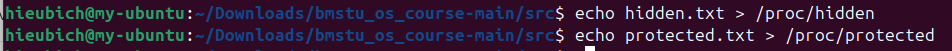
\includegraphics[scale=0.6]{img/proc.png}}
	\caption{Создание файлов, содержащих списки контроля доступа}
	\label{fig:proc}
\end{figure}

Файл hidden содержит имена файлов, которые необходимо скрыть полностью, файл protected ---  имена файлов, которые нельзя открывать, изменять, удалять.

После загрузки модуля содержимое рассматриваемой директории выглядит следующим образом (рисунок \ref{fig:ls_after}).

\begin{figure}[ph!]
	\center{
\includegraphics[scale=0.43]{img/ls_after.png}}
	\caption{Содержимое папки после загрузки модуля}
	\label{fig:ls_after}
\end{figure}

Результат выполнения команды ls не содержит файл hidden.txt.

После ввода пароля (рисунок \ref{fig:pass1}) файл hidden.txt перестает быть скрытым (рисунок \ref{fig:pass_after1}).

\clearpage

\begin{figure}[ph!]
	\center{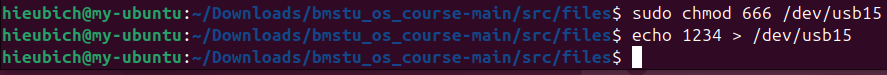
\includegraphics[scale=0.53]{img/pass1.png}}
	\caption{Ввод пароля}
	\label{fig:pass1}
\end{figure}


\begin{figure}[ph!]
	\center{
\includegraphics[scale=0.43]{img/ls_before.png}}
	\caption{Результат работы команды ls после ввода пароля}
	\label{fig:pass_after1}
\end{figure}

При попытке удалить файл protected.txt (рисунок \ref{fig:rm}) или вывести его содержимое с помощью cat ничего не происходит.

\begin{figure}[ph!]
	\center{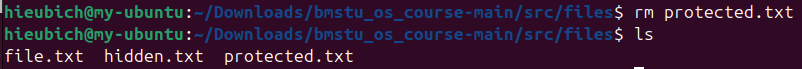
\includegraphics[scale=0.45]{img/rm.png}}
	\caption{Удаление файла protected.txt}
	\label{fig:rm}
\end{figure}

\begin{figure}[ph!]
	\center{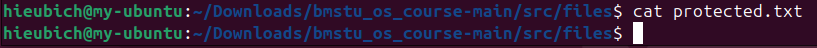
\includegraphics[scale=0.6]{img/cat.png}}
	\caption{Вывод содержимого файла protected.txt}
	\label{fig:cat1}
\end{figure}

После ввода пароля (рисунок \ref{fig:pass2}) операции над файлом protected.txt становятся возможными (рисунок \ref{fig:cat2}).

\begin{figure}[ph!]
	\center{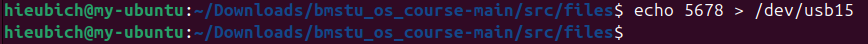
\includegraphics[scale=0.6]{img/pass2.png}}
	\caption{Ввод пароля}
	\label{fig:pass2}
\end{figure}

\begin{figure}[ph!]
	\center{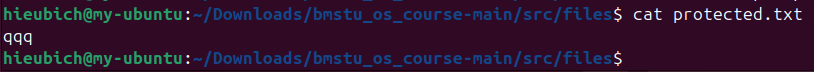
\includegraphics[scale=0.6]{img/cat_work.png}}
	\caption{Вывод содержимого файла protected.txt после ввода пароля}
	\label{fig:cat2}
\end{figure}




\backmatter %% Здесь заканчивается нумерованная часть документа и начинаются ссылки и
            
\Conclusion 

В ходе выполнения курсовой работы был определен способ перехвата системных вызовов --- путем регистрации функций перехвата с использованием ftrace, так как он позволяет перехватывать любые функции ядра и не требует его перекомпиляции. 

Для сокрытия файла была перехвачена функция getdents64, для запрета чтения из файла и записи в файл --- функции open, read и write, удаления --- unlink.%% заключение


% % Список литературы при помощи BibTeX
% Юзать так:
%
% pdflatex rpz
% bibtex rpz
% pdflatex rpz

\bibliographystyle{ugost2008}
\bibliography{rpz}


%%% Local Variables: 
%%% mode: latex
%%% TeX-master: "rpz"
%%% End: 


%
\appendix   % Тут идут приложения
%
\chapter{}

\begin{lstlisting}[label=code:main,caption=Файл main.c]
#include <linux/module.h>
#include <linux/kallsyms.h>
#include <linux/skbuff.h>
#include <linux/init.h>
#include <linux/fs.h>
#include <linux/device.h>
#include <linux/cdev.h>
#include <linux/proc_fs.h>
#include <linux/string.h>

#include "hooked.h"

MODULE_DESCRIPTION("OS 2024");
MODULE_AUTHOR("Pham Minh Hieu");
MODULE_LICENSE("GPL");

#define PROC_FILE_NAME_HIDDEN "hidden"
#define PROC_FILE_NAME_PROTECTED "protected"
#define PROC_DIR_NAME_PROTECTED "dir"

static char *buffer[MAX_BUF_SIZE];
char tmp_buffer[MAX_BUF_SIZE];
char hidden_files[100][50];
int hidden_index = 0;
char protected_files[100][50];
int protected_index = 0;
char protected_dirs[100][50];
int dir_index = 0;

static int read_index = 0;
static int write_index = 0;

static struct proc_dir_entry *proc_file_hidden;
static struct proc_dir_entry *proc_file_protected;
static struct proc_dir_entry *proc_dir_protected;

static ssize_t my_proc_write(struct file *file, const char __user *buf, size_t len, loff_t *ppos) 
{
    DMSG("my_proc_write called");

    if (len > MAX_BUF_SIZE - write_index + 1)
    {
        DMSG("buffer overflow");
        return -ENOSPC;
    }

    if (copy_from_user(&buffer[write_index], buf, len) != 0)
    {
        DMSG("copy_from_user fail");
        return -EFAULT;
    }

    write_index += len;
    buffer[write_index - 1] = '\0';

    if (strcmp(file->f_path.dentry->d_iname, PROC_FILE_NAME_HIDDEN) == 0)
    {
        snprintf(hidden_files[hidden_index], len, "%s", &buffer[write_index - len]);
        hidden_index++;
        DMSG("file written to hidden %s", hidden_files[hidden_index - 1]);
    }
    else if (strcmp(file->f_path.dentry->d_iname, PROC_FILE_NAME_PROTECTED) == 0)
    {
        snprintf(protected_files[protected_index], len, "%s", &buffer[write_index - len]);
        protected_index++;
        DMSG("file written to protected %s", protected_files[protected_index - 1]);
    }
    else if (strcmp(file->f_path.dentry->d_iname, PROC_DIR_NAME_PROTECTED) == 0)
    {
        snprintf(protected_dirs[dir_index], len, "%s", &buffer[write_index - len]);
        dir_index++;
        DMSG("file written to dir %s", protected_dirs[dir_index - 1]);
    }
    else
    {
        DMSG("Unknown file in proc %s", file->f_path.dentry->d_iname);
    }
    return len;
}

static ssize_t my_proc_read(struct file *file, char __user *buf, size_t len, loff_t *f_pos) 
{
    DMSG("my_proc_read called.\n");

    if (*f_pos > 0 || write_index == 0)
        return 0;

    if (read_index >= write_index)
        read_index = 0;

    int read_len = snprintf(tmp_buffer, MAX_BUF_SIZE, "%s\n", &buffer[read_index]);
    if (copy_to_user(buf, tmp_buffer, read_len) != 0)
    {
        DMSG("copy_to_user error.\n");
        return -EFAULT;
    }

    read_index += read_len;
    *f_pos += read_len;

    return read_len;
}

static const struct proc_ops fops =
{
    proc_read: my_proc_read,
    proc_write: my_proc_write
}; 


static int fh_init(void)
{
    DMSG("call init");

	proc_file_hidden = proc_create(PROC_FILE_NAME_HIDDEN, S_IRUGO | S_IWUGO, NULL, &fops);
  	if (!proc_file_hidden) 
        return -ENOMEM;

    proc_file_protected = proc_create(PROC_FILE_NAME_PROTECTED, S_IRUGO | S_IWUGO, NULL, &fops);
    if (!proc_file_protected) 
	{
        remove_proc_entry(PROC_FILE_NAME_HIDDEN, NULL);
        return -ENOMEM;
    }

    proc_dir_protected = proc_create(PROC_DIR_NAME_PROTECTED, S_IRUGO | S_IWUGO, NULL, &fops);
    if (!proc_dir_protected) 
	{
        remove_proc_entry(PROC_FILE_NAME_HIDDEN, NULL);
        remove_proc_entry(PROC_FILE_NAME_PROTECTED, NULL);
        return -ENOMEM;
    }
	DMSG("proc file created");

    if (start_hook_resources() != 0)
    {
        remove_proc_entry(PROC_FILE_NAME_HIDDEN, NULL);
        remove_proc_entry(PROC_FILE_NAME_PROTECTED, NULL);
        remove_proc_entry(PROC_DIR_NAME_PROTECTED, NULL);
        DMSG("Problem in hook functions");
        return -1;
    }

    return 0;
}


static void fh_exit(void)
{
    remove_proc_entry(PROC_FILE_NAME_HIDDEN, NULL);
    remove_proc_entry(PROC_FILE_NAME_PROTECTED, NULL);
    remove_proc_entry(PROC_DIR_NAME_PROTECTED, NULL);
    fh_remove_hooks(demo_hooks, ARRAY_SIZE(demo_hooks));
    DMSG("called exit module");
}

module_init(fh_init);
module_exit(fh_exit);

\end{lstlisting}


\begin{lstlisting}[label=code:hook1,caption=Файл hook.h]
#include <linux/ftrace.h>
#include <linux/kallsyms.h>
#include <linux/syscalls.h>
#include <linux/kernel.h>
#include <linux/version.h>
#include <linux/kprobes.h>
#include <linux/delay.h>
#include <linux/kthread.h>
#include <linux/kernel.h>
#include <asm/signal.h>
#include <linux/delay.h>
#include <linux/fcntl.h>
#include <linux/types.h>
#include <linux/dirent.h>
#include <linux/device.h>
#include <linux/cdev.h>
#include <linux/module.h>
#include <linux/init.h>
#include <linux/fs.h>
#include <linux/proc_fs.h>

#define FILE_NAME (strrchr(__FILE__, '/') ? strrchr(__FILE__, '/') + 1 : __FILE__)
#define DMSG(msg_fmt, msg_args...) \
    printk(KERN_INFO "OS: %s(%04u): " msg_fmt "\n", FILE_NAME, __LINE__, ##msg_args)

#define MAX_BUF_SIZE 1000

extern char hidden_files[100][50];
extern int hidden_index;
extern char protected_files[100][50];
extern int protected_index;
extern char protected_dirs[100][50];
extern int dir_index;

int check_fs_blocklist(char *input);
int check_fs_hidelist(char *input);
int check_dir_blocklist(char *input);


static unsigned long lookup_name(const char *name)
{
    struct kprobe kp = {
        .symbol_name = name
    };
    unsigned long retval;

    if (register_kprobe(&kp) < 0) 
    {
        DMSG("register_kprobe failed for %s", name);
        return 0;
    }
    retval = (unsigned long) kp.addr;
    unregister_kprobe(&kp);
    return retval;
}


#define USE_FENTRY_OFFSET 0

struct ftrace_hook {
    const char *name;
    void *function;
    void *original;

    unsigned long address;
    struct ftrace_ops ops;
};

static int fh_resolve_hook_address(struct ftrace_hook *hook)
{
    hook->address = lookup_name(hook->name);

    if (!hook->address) {
        pr_debug("unresolved symbol: %s\n", hook->name);
        return -ENOENT;
    }

    *((unsigned long*) hook->original) = hook->address + MCOUNT_INSN_SIZE;

    return 0;
}

static void notrace fh_ftrace_thunk(unsigned long ip, unsigned long parent_ip,
                                    struct ftrace_ops *ops, struct ftrace_regs *fregs)
{
    struct pt_regs *regs = ftrace_get_regs(fregs);
    struct ftrace_hook *hook = container_of(ops, struct ftrace_hook, ops);

    regs->ip = (unsigned long)hook->function;
}

int fh_install_hook(struct ftrace_hook *hook);
void fh_remove_hook(struct ftrace_hook *hook);
int fh_install_hooks(struct ftrace_hook *hooks, size_t count);
void fh_remove_hooks(struct ftrace_hook *hooks, size_t count);

#define PTREGS_SYSCALL_STUBS 1


static char *get_filename(const char __user *filename)
{
    char *kernel_filename=NULL;

    kernel_filename = kmalloc(4096, GFP_KERNEL);
    if (!kernel_filename)
        return NULL;

    if (strncpy_from_user(kernel_filename, filename, 4096) < 0) {
        kfree(kernel_filename);
        return NULL;
    }

    return kernel_filename;
}


static asmlinkage long (*real_sys_getdents64)(const struct pt_regs *);

static asmlinkage int fh_sys_getdents64(const struct pt_regs *regs)
{
    struct linux_dirent64 __user *dirent = (struct linux_dirent64 *)regs->si;
    struct linux_dirent64 *previous_dir, *current_dir, *dirent_ker = NULL;
    unsigned long offset = 0;
    int ret = real_sys_getdents64(regs);

    dirent_ker = kzalloc(ret, GFP_KERNEL);

    if ((ret <= 0) || (dirent_ker == NULL))
    {
        return ret;
    }

    long error;
    error = copy_from_user(dirent_ker, dirent, ret);

    if (error)
    {
        kfree(dirent_ker);
        return ret;
    }

    while (offset < ret)
    {
        current_dir = (void *)dirent_ker + offset;

        if (check_fs_hidelist(current_dir->d_name))
        {
            if (current_dir == dirent_ker)
            {
                ret -= current_dir->d_reclen;
                memmove(current_dir, (void *)current_dir + current_dir->d_reclen, ret);
                continue;
            }

            previous_dir->d_reclen += current_dir->d_reclen;
        }
        else
        {
            previous_dir = current_dir;
        }

        offset += current_dir->d_reclen;
    }

    error = copy_to_user(dirent, dirent_ker, ret);
    if (error)
    {
        DMSG("copy_to_user error");
    }

    kfree(dirent_ker);
    return ret;
}

static asmlinkage long (*real_sys_rename)(struct pt_regs *regs);

static asmlinkage long fh_sys_rename(struct pt_regs *regs)
{
    long ret=0;
    char *kernel_filename = get_filename((void*) regs->si);

    if (check_fs_blocklist(kernel_filename) || check_dir_blocklist(kernel_filename))
    {

        pr_info("blocked to not rename file : %s\n", kernel_filename);
        kfree(kernel_filename);
        return -EPERM;

    }

    kfree(kernel_filename);
    ret = real_sys_rename(regs);

    return ret;
}



static asmlinkage long (*real_sys_open)(struct pt_regs *regs);

static asmlinkage long fh_sys_open(struct pt_regs *regs)
{
	char *kernel_filename;
	kernel_filename = get_filename((void*) regs->si);

	if (check_fs_blocklist(kernel_filename))
	{
		DMSG("block open file : %s", kernel_filename);
		kfree(kernel_filename);
		return -EPERM;
	}

	kfree(kernel_filename);

	return real_sys_open(regs);
}


static asmlinkage long (*real_sys_unlink) (struct pt_regs *regs);

static asmlinkage long fh_sys_unlink(struct pt_regs *regs)
{
    char *kernel_filename = get_filename((void*) regs->si);

    if (check_fs_blocklist(kernel_filename) || check_dir_blocklist(kernel_filename))
    {

        pr_info("blocked to not remove file : %s\n", kernel_filename);
        kfree(kernel_filename);
        return -EPERM;

    }

    kfree(kernel_filename);
    return real_sys_unlink(regs);
}

#define SYSCALL_NAME(name) ("__x64_" name)

#define HOOK(_name, _function, _original)	\
{					\
.name = SYSCALL_NAME(_name),	\
.function = (_function),	\
.original = (_original),	\
}

static struct ftrace_hook demo_hooks[] = {
    HOOK("sys_open", fh_sys_open, &real_sys_open),
    HOOK("sys_unlink", fh_sys_unlink, &real_sys_unlink),
    HOOK("sys_rename", fh_sys_rename, &real_sys_rename),
    HOOK("sys_getdents64", fh_sys_getdents64, &real_sys_getdents64)
};


static int start_hook_resources(void)
{
    int err;
    err = fh_install_hooks(demo_hooks, ARRAY_SIZE(demo_hooks));
    if (err)
    {
        return err;
    }
    return 0;
}

\end{lstlisting}
\begin{lstlisting}[label=code:hook2,caption=Файл hook.c]
#include "hooked.h"

int check_dir_blocklist(char *input)
{
    int i = 0;

    while (i != dir_index)
    {
        if(strstr(input,  protected_dirs[i]) != NULL)
            return 1;
        i++;
    }

    return 0;
}

int check_fs_blocklist(char *input)
{
    int i = 0;

    while (i != protected_index)
    {
        if(strstr(input, protected_files[i]) != NULL)
            return 1;
        i++;
    }

    return 0;
}

int check_fs_hidelist(char *input)
{
    int i = 0;

    while (i != hidden_index)
    {
        if(strstr(input, hidden_files[i]) != NULL)
            return 1;
        i++;
    }

    return 0;
}

int fh_install_hook(struct ftrace_hook *hook)
{
    int error;

    error = fh_resolve_hook_address(hook);
    if (error)
    {
        return error;
    }

    hook->ops.func = fh_ftrace_thunk;
    hook->ops.flags = FTRACE_OPS_FL_SAVE_REGS
    | FTRACE_OPS_FL_RECURSION
    | FTRACE_OPS_FL_IPMODIFY;

    error = ftrace_set_filter_ip(&hook->ops, hook->address, 0, 0);
    if (error) 
    {
        DMSG("ftrace_set_filter_ip() failed: %d\n", error);
        return error;
    }

    error = register_ftrace_function(&hook->ops);
    if (error) 
    {
        DMSG("register_ftrace_function() failed: %d\n", error);
        ftrace_set_filter_ip(&hook->ops, hook->address, 1, 0);
        return error;
    }

    return 0;
}


void fh_remove_hook(struct ftrace_hook *hook)
{
    int err;

    err = unregister_ftrace_function(&hook->ops);
    if (err) 
    {
        DMSG("unregister_ftrace_function() failed: %d\n", err);
    }

    err = ftrace_set_filter_ip(&hook->ops, hook->address, 1, 0);
    if (err) 
    {
        DMSG("ftrace_set_filter_ip() failed: %d\n", err);
    }
}


int fh_install_hooks(struct ftrace_hook *hooks, size_t count)
{
    int err;
    size_t i;

    for (i = 0; i < count; i++) 
    {
        err = fh_install_hook(&hooks[i]);
        if (err)
        {
            while (i != 0) 
            {
                fh_remove_hook(&hooks[--i]);
            }
            return err;
        }
    }

    return 0;
}


void fh_remove_hooks(struct ftrace_hook *hooks, size_t count)
{
    size_t i;

    for (i = 0; i < count; i++)
    {
        fh_remove_hook(&hooks[i]);
    }
}

\end{lstlisting}
%
%\include{91-appendix2}

\end{document}

%%% Local Variables:
%%% mode: latex
%%% TeX-master: t
%%% End:
